\documentclass{article}
% translate with >> pdflatex -shell-escape <file>

% This file is an extract of the PGFPLOTS manual, copyright by Christian Feuersaenger.
% 
% Feel free to use it as long as you cite the pgfplots manual properly.
%
% See
%   http://pgfplots.sourceforge.net/pgfplots.pdf
% for the complete manual.
%
% Any required input files (for <plot table> or <plot file> or the table package) can be downloaded
% at
% http://www.ctan.org/tex-archive/graphics/pgf/contrib/pgfplots/doc/latex/
% and
% http://www.ctan.org/tex-archive/graphics/pgf/contrib/pgfplots/doc/latex/plotdata/

\usepackage{pgfplots}
\pgfplotsset{compat=newest}

\pagestyle{empty}

\usepgfplotslibrary{ternary}

\begin{document}
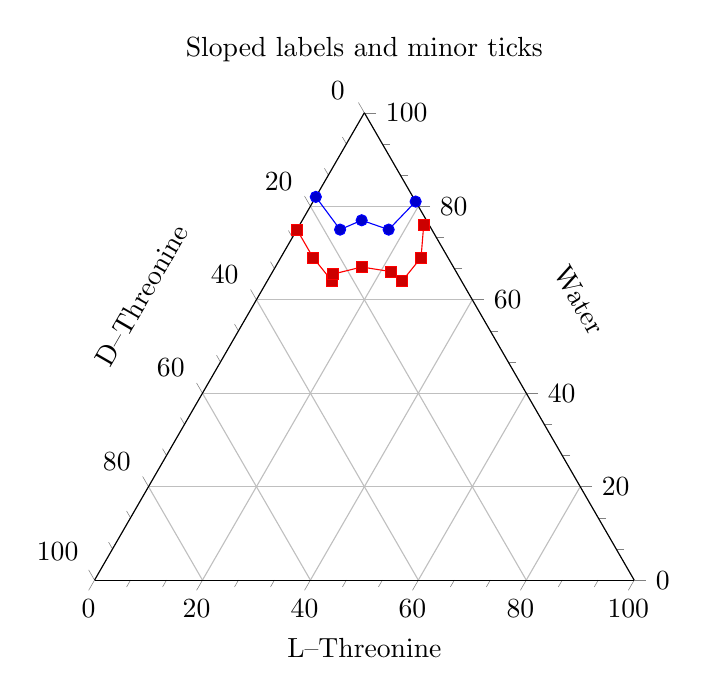
\begin{tikzpicture}
\begin{ternaryaxis}[
	title=Sloped labels and minor ticks,
	xlabel=Water,
	ylabel=D--Threonine,
	zlabel=L--Threonine,
	label style={sloped},
	minor tick num=2,
]
	\addplot3 coordinates {
        (0.82,  0.18,  0.00)
        (0.75,  0.17,  0.08)
        (0.77,  0.12,  0.11)
        (0.75,  0.08,  0.17)
        (0.81,  0.00,  0.19)
	};
	\addplot3 coordinates {
        (0.75,  0.25,  0.00)
        (0.69,  0.25,  0.06)
        (0.64,  0.24,  0.12)
        (0.655, 0.23,  0.115)
        (0.67,  0.17,  0.16)
        (0.66,  0.12,  0.22)
        (0.64,  0.11,  0.25)
        (0.69,  0.05,  0.26)
        (0.76,  0.01,  0.23)
	};
\end{ternaryaxis}
\end{tikzpicture}
\end{document}
